\documentclass[11pt,a4paper]{article}
\usepackage[T1]{fontenc}
\usepackage[utf8]{inputenc}
\usepackage{lmodern}
\usepackage[margin=2.3cm]{geometry}
\usepackage{amsmath,amssymb,bm}
\usepackage{booktabs,tabularx}
\usepackage{graphicx}
\usepackage{upgreek}
\usepackage{xcolor}
\usepackage{tikz}
\usetikzlibrary{arrows.meta,decorations.pathmorphing,calc}
\usepackage[colorlinks=true,linkcolor=blue!50!black,citecolor=blue!50!black,urlcolor=blue!50!black]{hyperref}
\usepackage{caption}
\captionsetup{font=small,labelfont=bf}
\graphicspath{{figures/}}

\newcommand{\ket}[1]{|#1\rangle}
\newcommand{\bra}[1]{\langle #1|}
\newcommand{\gp}{\ket{g_p}}
\newcommand{\gc}{\ket{g_c}}
\newcommand{\Om}{\Omega}
\newcommand{\etap}{\eta_\perp}
\newcommand{\etasp}{\eta_{\rm sp}}
\newcommand{\nur}{\nu_r}
\newcommand{\micro}{\upmu}
\newcommand{\SI}[2]{\ensuremath{#1\,\mathrm{#2}}}

\title{Anomalous Fock statistics and a Sisyphus channel\\in radial EIT cooling at an LP$_{11}$ node\\[3pt]
\large Theory notes --- working draft}
\author{}
\date{7 November 2026}

\begin{document}
\maketitle

\begin{abstract}
Radial EIT cooling with the probe in the LP$_{11}$ mode of a hollow-core fibre and the coupling beam in LP$_{01}$ has, in a soft trap, three regimes of energy removal from a trapped atom. They are separated by the saturation of the $n\to n-1$ sideband, at $s\,n=1$, and by the point where the Raman coupling exceeds the trap frequency, at $s\,n=2(\nur/\Gamma_n)^2$. Between the two, the removal rate is constant while recoil spreads the energy by $\propto\sqrt n$ quanta per photon. The steady state then develops a power-law tail $P(n)\propto n^{-\mu}$, whose exponent is set by $h$, the recoil energy per removed phonon: a minimal model gives $\mu\simeq1/h$. Above the second crossover the atom follows the position-dependent dark state of the LP$_{11}$ profile, and a Sisyphus-like channel removes energy at a rate that grows with $n$. We show why each ingredient is a consequence of the node geometry, give the scales and thresholds, and list the tests still needed. Master-equation diagnostics support the regime structure and the power-law tail. The thresholds and the mechanism of the fast channel are hypotheses at this stage.
\end{abstract}

\tableofcontents

%=====================================================================
\section{Status and motivation}
%=====================================================================
This note grew out of a numerical problem. For case A of the fibre paper (core radius $a=\SI{15}{\micro m}$, $\nur=7.15$\,kHz, $\etasp=0.71$), the master-equation steady state needs very large Fock truncations $N$. Case B ($a=3.5\,\mu$m, $\etasp=0.34$) is converged at $N=20$. The convergence is worst at intermediate saturation, $s\approx0.1$, where $n_{\rm ss}$ still grows by 0.7\% between $N=300$ and 400. It is better at both smaller and larger $s$. All numbers below are for case A, $^{87}$Rb D1, $\Delta=3\Gamma$, unless stated otherwise. They were obtained with the eliminated, banded master equation of the fibre project (\texttt{simulation/results/convergence/}).

The status of each statement is marked:
\begin{itemize}
\item \textbf{[numerics]} --- computed with the master equation and checked for convergence;
\item \textbf{[model]} --- derived from the minimal model of Sec.~\ref{sec:model};
\item \textbf{[hypothesis]} --- a proposed explanation that still needs a dedicated test.
\end{itemize}

%=====================================================================
\section{Setting}
\label{sec:setting}
%=====================================================================
The probe, in LP$_{11}$, couples $\gp$ to the excited state with a field that vanishes on the axis and grows linearly near it, $f_p(\hat x)\simeq G_{11}\hat x/a$. The coupling beam, in LP$_{01}$, couples $\gc$ with an almost flat profile. With the EIT condition $\Om_c^2=4\nur(\Delta+\nur)$, the light-shifted $\gc$ forms a narrow resonance at the red sideband, $\delta_+=\nur$, with width
\begin{equation}
  \Gamma_n\simeq\Gamma\frac{\Om_c^2}{4\Delta^2}\simeq\frac{\Gamma}{\Delta}\,\nur\qquad(\Gamma_n/\nur=0.333\ \text{for}\ \Delta=3\Gamma).
\end{equation}
The adiabatic elimination of the excited state is accurate here (Ref.~\cite{reiter2012}; $<0.5\%$ against the full master equation). It turns the problem into a Raman problem on $\{\gp,\gc\}\otimes$ motion. The relevant parameters are collected in Table~\ref{tab:params}.

\begin{table}[h]
\centering\small
\caption{Parameters. Case A values for $^{87}$Rb D1, $\Delta=3\Gamma$, $b_p=1/2$.}
\label{tab:params}
\begin{tabularx}{\textwidth}{@{}llX@{}}
\toprule
Symbol & Case A & Meaning\\
\midrule
$\etap=G_{11}x_0/a$ & 0.021 & Lamb--Dicke parameter of the drive (scale $a$)\\
$\etasp=kx_0$ & 0.71 & Lamb--Dicke parameter of a spontaneous photon (scale $\lambda$); $\etasp^2=\omega_{\rm rec}/\nur$\\
$s=2\Om_\perp^2/\Gamma\Gamma_n$ & --- & saturation of the $1\to0$ sideband, $\Om_\perp=\etap\bar\Om_p$\\
$\Om_R=\Om_c\Om_\perp/2\Delta$ & $\Om_R^2=s\Gamma_n^2/2$ & Raman coupling $\ket{g_p,n}\leftrightarrow\ket{g_c,n-1}$, per $\sqrt n$\\
$\kappa=1/b_p$ & 2 & photons per cooling cycle\\
$\alpha=\langle u^2\rangle$ & 0.40 & mean square of $u=\hat{\mathbf k}\cdot\hat{\mathbf x}$, the projection of the emission direction on $x$\\
$h=\kappa\alpha\etasp^2$ & 0.40 & recoil quanta added per removed phonon\\
$U_0/\hbar\nur$ & 1552 & trap depth in radial quanta\\
\bottomrule
\end{tabularx}
\end{table}

%=====================================================================
\section{Why the LP$_{11}$ node is special}
\label{sec:special}
%=====================================================================
Five properties of the fibre geometry combine. Each is unusual on its own, and together they are what makes the statistics anomalous. Figure~\ref{fig:mechanism} summarises the resulting mechanism.

\paragraph{(i) The motional ground state is dark.} At the node the carrier vanishes, so the probe drives only sidebands. From $\ket{g_p,0}$ the only allowed process is the blue sideband, suppressed by $(\Gamma/4\Delta)^2$~\cite{morigi2000}. The atom in the ground state therefore hardly scatters. This is the fibre analogue of an ion at a standing-wave node~\cite{cirac1992}, a dark state in Fock space at the bottom of the ladder.

\paragraph{(ii) The coupling grows with $n$.} The sideband matrix element is $\langle n-1|\hat x|n\rangle=x_0\sqrt n$, so level $n$ sees the effective saturation
\begin{equation}
  s_n=s\,n .
  \label{eq:sn}
\end{equation}
In a carrier-present scheme the carrier dominates and its scattering does not depend on $n$. At the node all scattering is sideband scattering, so cold atoms scatter little and hot atoms a lot: the scattering is \emph{energy-selective}.

\paragraph{(iii) The drive and the recoil live on separate length scales.} The drive varies on the mode scale $a$, the photon recoil on the optical scale $\lambda$:
\begin{equation}
  \frac{\etap}{\etasp}=\frac{G_{11}}{ka}\approx0.03 .
\end{equation}
Each absorption therefore removes exactly one quantum ($\etap\ll1$, deep Lamb--Dicke regime). Each emission, instead, kicks the atom far outside the Lamb--Dicke regime. For the displacement $e^{i\etasp u(\hat b+\hat b^\dagger)}$ acting on $\ket n$ the jump statistics are exact:
\begin{equation}
  \langle\Delta n\rangle=\etasp^2u^2,\qquad {\rm Var}(\Delta n)=\etasp^2u^2(2n+1).
  \label{eq:kick}
\end{equation}
Here $u=\hat{\mathbf k}\cdot\hat{\mathbf x}=\sin\vartheta\cos\varphi$ is the projection of the emission direction $\hat{\mathbf k}$ of the spontaneous photon (polar angle $\vartheta$, azimuth $\varphi$) on the cooled radial axis $x$: the photon carries momentum $\hbar k$, of which $\hbar k u$ along $x$, and the displacement $e^{i\etasp u(\hat b+\hat b^\dagger)}=e^{iku\hat x}$ is that momentum kick. $u$ is random from photon to photon, distributed according to the dipole radiation pattern; for a dipole perpendicular to $x$ its mean square is $\alpha=\langle u^2\rangle=2/5$ (Table~\ref{tab:params}; the code uses a ten-node quadrature of this distribution, $\langle u^2\rangle=0.397$). Averaged over $u$, one photon thus gives $\langle\Delta n\rangle=\alpha\etasp^2$ and ${\rm Var}(\Delta n)\simeq\alpha\etasp^2(2n+1)$. The spread grows as $\sqrt n$ while the mean stays fixed (Fig.~\ref{fig:recoil}). This is multiplicative noise: a hot atom is kicked by many quanta in a random direction, while the cooling step is always one quantum. In ion-trap EIT cooling both Lamb--Dicke parameters are of order 0.1 and this separation does not occur.

\begin{figure}[t]
\centering
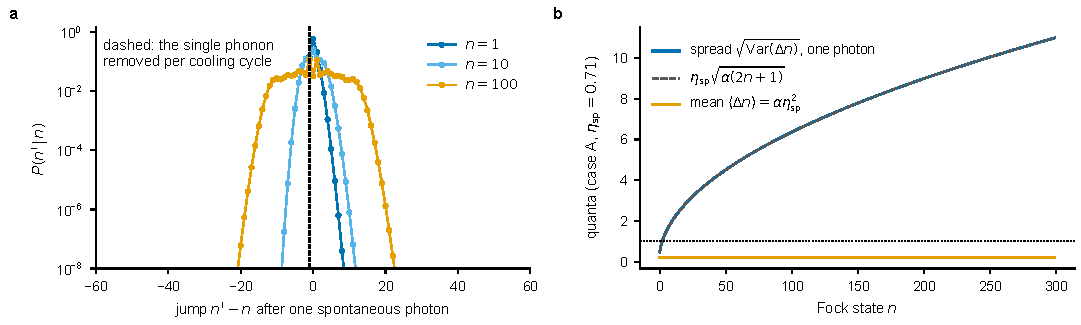
\includegraphics[width=\textwidth]{recoil.pdf}
\caption{Recoil statistics of one spontaneous photon (case A). \textbf{a}, exact distribution of the jump $n\to n'$, averaged over the emission pattern, for $n=1$, 10, 100; the cooling step is a single quantum (dashed). \textbf{b}, spread and mean of the jump against $n$: the spread grows as $\etasp\sqrt{\alpha(2n+1)}$, Eq.~\eqref{eq:kick}, while the mean is fixed at $\alpha\etasp^2$.}
\label{fig:recoil}
\end{figure}

\paragraph{(iv) The trap is soft on the recoil scale.} The radial confinement comes from the LP$_{01}$ waist $w\approx0.67a\gg\lambda$, so $\nur\propto1/a$ is comparable to the recoil frequency of the cooling photon:
\begin{equation}
  h=\kappa\alpha\etasp^2=\frac{\kappa\alpha\,\omega_{\rm rec}}{\nur}\approx0.4\quad\text{(case A)}.
\end{equation}
Each removed phonon therefore costs almost half a phonon of recoil. This is the parameter that controls the tail (Sec.~\ref{sec:model}).

\paragraph{(v) The dark state rotates along the mode profile.} With the excited state eliminated, the ground manifold has a dark state and a bright state,
\begin{equation}
  \ket{D(x)}=\cos\theta\,\gp-\sin\theta\,\gc,\qquad \tan\theta(x)=\frac{\bar\Om_pf_p(x)}{\Om_c}\simeq\frac{\Gamma_n}{\nur}\sqrt{\frac s8}\,\frac{x}{x_0},
  \label{eq:theta}
\end{equation}
where the last form uses the near-axis profile and the EIT condition. The orthogonal combination is the bright state,
\begin{equation}
  \ket{B(x)}=\sin\theta\,\gp+\cos\theta\,\gc .
  \label{eq:bright}
\end{equation}

\emph{Why the bright state has this light shift.} Both lasers drive the same excited state $\ket e$. At a fixed position $x$ (motion neglected), the coupling from the ground manifold to $\ket e$ is the operator
\begin{equation}
  A(x)=\tfrac12\big[\bar\Om_pf_p(x)\,\bra{g_p}+\Om_c\,\bra{g_c}\big],\qquad
  A\ket{D}=0,\qquad A\ket{B}=\tfrac12\Om_{\rm eff}(x),\qquad
  \Om_{\rm eff}^2=\Om_c^2+\bar\Om_p^2f_p(x)^2 .
\end{equation}
The dark state is the combination for which the two excitation amplitudes cancel, so it is not coupled to $\ket e$ at all. The bright state couples with the total Rabi frequency $\Om_{\rm eff}$. Eliminating $\ket e$ adiabatically (detuning $\Delta$, width $\Gamma$; Ref.~\cite{reiter2012}) gives the effective Hamiltonian $\frac{\Delta}{\Delta^2+\Gamma^2/4}A^\dagger A$ and an optical-pumping rate $\frac{\Gamma}{\Delta^2+\Gamma^2/4}A^\dagger A$. Both act only on $\ket B$. For $\Delta\gg\Gamma$ the bright state therefore has the second-order light shift and width
\begin{equation}
  \delta_B(x)=\frac{\Om_c^2+\bar\Om_p^2f_p(x)^2}{4\Delta},\qquad
  \Gamma_B(x)=\Gamma\,\frac{\Om_c^2+\bar\Om_p^2f_p(x)^2}{4\Delta^2},
  \label{eq:dB0}
\end{equation}
while $\ket D$ has neither shift nor width. The shift is positive, i.e.\ $\ket B$ is pushed up, because the lasers are blue-detuned ($\Delta>0$): in the frame rotating with the lasers the excited state lies $\hbar\Delta$ \emph{below} the ground manifold, and level repulsion pushes the state coupled to it upwards (for red detuning the shift would be negative). On the axis, $f_p(0)=0$, so $\ket B=\gc$, $\delta_B(0)=\Om_c^2/4\Delta=\nur$ by the EIT condition and $\Gamma_B(0)=\Gamma_n$: the bright state at the node is the narrow dressed state of EIT cooling. Away from the axis the probe intensity $\propto f_p(x)^2$ adds to the shift, so the bright state sits on a hill,
\begin{equation}
  \delta_B(x)-\delta_B(0)=\frac{\bar\Om_p^2f_p(x)^2}{4\Delta}\simeq\hbar\nur\Big(\frac{\Gamma_n}{\nur}\Big)^2\frac{s}{8}\Big(\frac{x}{x_0}\Big)^2
  =\hbar\nur\tan^2\theta(x),
  \label{eq:dB}
\end{equation}
where the near-axis form uses $\bar\Om_pf_p\simeq\Om_\perp x/x_0$, $\Om_\perp^2=s\Gamma\Gamma_n/2$, $\Om_c^2\simeq4\nur\Delta$ and $\Gamma/\Delta=\Gamma_n/\nur$.
The hill grows as $x^2$, like the trap, and extends smoothly over the whole core (Fig.~\ref{fig:geometry}). In free-space gray molasses the light shift is modulated on the scale $\lambda/2$.

\begin{figure}[t]
\centering
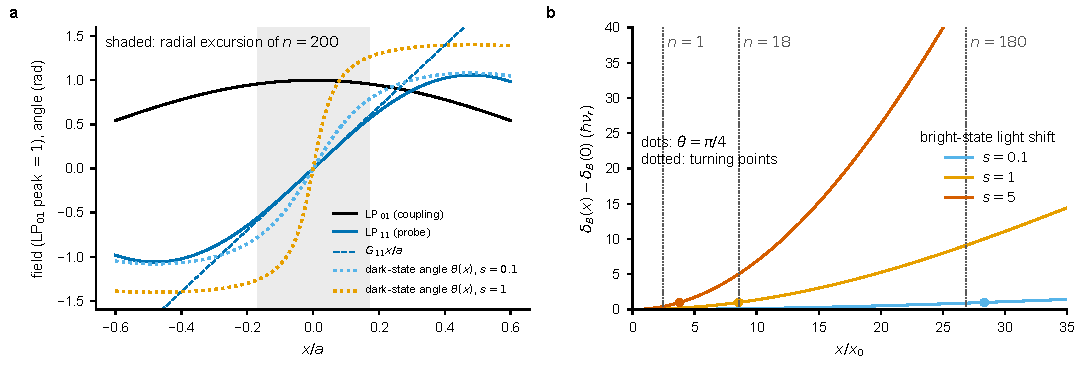
\includegraphics[width=\textwidth]{geometry.pdf}
\caption{The LP$_{11}$ node. \textbf{a}, LP$_{01}$ and LP$_{11}$ profiles at equal power and the dark-state angle $\theta(x)$, Eq.~\eqref{eq:theta}, for $s=0.1$ and 1. Shaded: radial excursion of $n=200$. \textbf{b}, bright-state light-shift hill, Eq.~\eqref{eq:dB}, for $s=0.1$, 1 and 5. Dots mark $\theta=\pi/4$; dotted lines are the turning points $x_t=2x_0\sqrt n$ of $n=1$, 18 and 180. The dot of each $s$ falls on the turning point of $n=18/s$, the onset of regime III (Sec.~\ref{sec:sisyphus}).}
\label{fig:geometry}
\end{figure}

\begin{table}[h]
\centering\small
\caption{EIT cooling of a tightly trapped ion versus radial EIT cooling at an LP$_{11}$ node.}
\label{tab:contrast}
\begin{tabularx}{\textwidth}{@{}lXX@{}}
\toprule
& tightly trapped ion & LP$_{11}$ node in a fibre\\
\midrule
carrier & present (suppressed at the dark resonance) & absent (node): dark ground state\\
scattering & dominated by the $n$-independent carrier & sideband only, grows with $n$\\
drive / recoil scales & both $\sim\lambda$, $\eta\sim0.1$ & $a$ vs $\lambda$: $\etap\approx0.02$, $\etasp\approx0.7$\\
recoil per phonon $h$ & $\ll1$ & $\approx0.4$ (soft trap)\\
spatial structure of the dark state & on the scale $\lambda$ (if any) & on the scale $a$, commensurate with the trap\\
\bottomrule
\end{tabularx}
\end{table}


\begin{figure}[t]
\centering
\resizebox{\textwidth}{!}{%
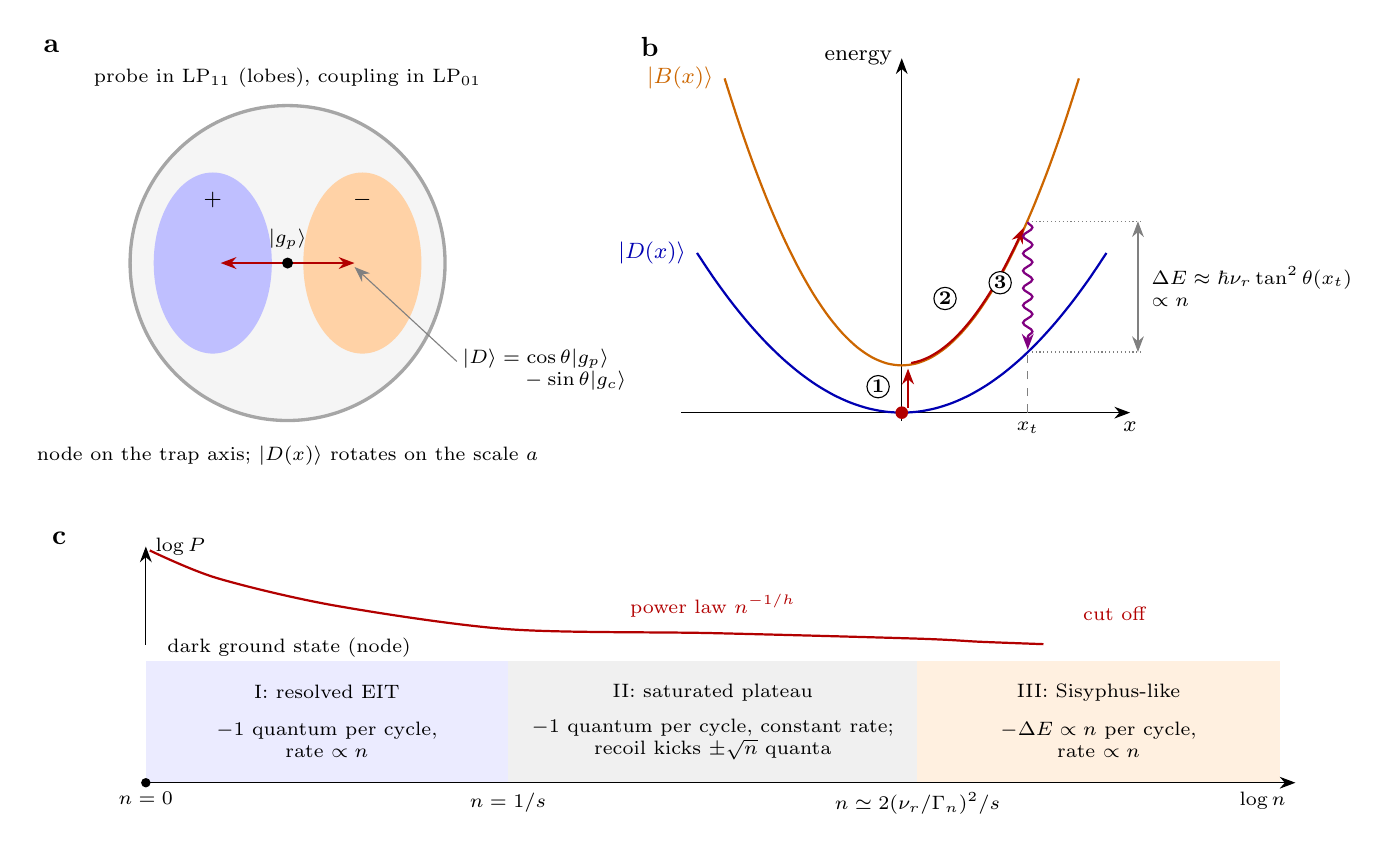
\begin{tikzpicture}[font=\footnotesize, >={Stealth[length=2mm]},
  stp/.style={circle, draw, inner sep=0.6pt, font=\scriptsize\bfseries, fill=white}]
% ======================= (a) fibre cross-section =======================
\begin{scope}
  \node[font=\bfseries\normalsize] at (-3.0,2.75) {a};
  \node[font=\scriptsize, align=center] at (0,2.35) {probe in LP$_{11}$ (lobes), coupling in LP$_{01}$};
  \fill[gray!8] (0,0) circle (2);
  \draw[gray!70, line width=1.2pt] (0,0) circle (2);
  \fill[blue!25] (-0.95,0) ellipse (0.75 and 1.15);
  \fill[orange!35] (0.95,0) ellipse (0.75 and 1.15);
  \node at (-0.95,0.8) {$+$};
  \node at (0.95,0.8) {$-$};
  \draw[red!70!black, <->, thick] (-0.85,0) -- (0.85,0);
  \fill[black] (0,0) circle (0.07);
  \node[font=\scriptsize] at (0,0.3) {$\ket{g_p}$};
  \draw[->, gray] (2.15,-1.25) -- (0.85,-0.05);
  \node[font=\scriptsize, align=left, anchor=west] at (2.1,-1.35) {$\ket{D}=\cos\theta\ket{g_p}$\\$\phantom{\ket{D}=}-\sin\theta\ket{g_c}$};
  \node[font=\scriptsize, align=center] at (0,-2.45) {node on the trap axis; $\ket{D(x)}$ rotates on the scale $a$};
\end{scope}
% ======================= (b) Sisyphus cycle =======================
\begin{scope}[shift={(7.8,-1.9)}]
  \node[font=\bfseries\normalsize] at (-3.2,4.65) {b};
  \draw[->] (-2.8,0) -- (2.9,0) node[below] {$x$};
  \draw[->] (0,-0.1) -- (0,4.5) node[left] {energy};
  \draw[thick, blue!70!black, domain=-2.6:2.6, smooth, variable=\x] plot (\x, {0.3*\x*\x});
  \draw[thick, orange!80!black, domain=-2.25:2.25, smooth, variable=\x] plot (\x, {0.6+0.72*\x*\x});
  \node[blue!70!black, anchor=east] at (-2.62,2.03) {$\ket{D(x)}$};
  \node[orange!80!black, anchor=east] at (-2.27,4.25) {$\ket{B(x)}$};
  % cycle
  \fill[red!70!black] (0,0) circle (0.08);
  \draw[->, red!70!black, thick] (0.08,0.06) -- (0.08,0.56);
  \node[stp] at (-0.3,0.33) {1};
  \draw[->, red!70!black, thick, domain=0.12:1.55, smooth, variable=\x] plot (\x, {0.62+0.72*\x*\x});
  \node[stp] at (0.55,1.45) {2};
  \draw[->, decorate, decoration={snake, amplitude=0.6mm, segment length=2.2mm, post length=1.6mm},
        violet, thick] (1.6,2.42) -- (1.6,0.8);
  \node[stp] at (1.25,1.65) {3};
  \draw[gray, densely dotted] (1.65,0.77) -- (3.05,0.77);
  \draw[gray, densely dotted] (1.65,2.43) -- (3.05,2.43);
  \draw[<->, gray] (3.0,0.77) -- (3.0,2.43);
  \node[anchor=west, font=\scriptsize, align=left] at (3.05,1.6) {$\Delta E\approx\hbar\nur\tan^2\theta(x_t)$\\$\propto n$};
  \draw[gray, dashed] (1.6,0) -- (1.6,0.77);
  \node[below, font=\scriptsize] at (1.6,0) {$x_t$};
\end{scope}
% ======================= (c) regimes along the Fock ladder =======================
\begin{scope}[shift={(-2.4,-6.6)}]
  \node[font=\bfseries\normalsize] at (-0.5,3.1) {c};
  \fill[blue!8] (0.6,0) rectangle (5.2,1.55);
  \fill[gray!12] (5.2,0) rectangle (10.4,1.55);
  \fill[orange!12] (10.4,0) rectangle (15.0,1.55);
  \draw[->] (0.6,0) -- (15.2,0) node[below left, font=\scriptsize] {$\log n$};
  \fill[black] (0.6,0) circle (0.06);
  \node[below, font=\scriptsize] at (0.6,0) {$n=0$};
  \node[below, font=\scriptsize] at (5.2,0) {$n=1/s$};
  \node[below, font=\scriptsize] at (10.4,0) {$n\simeq2(\nur/\Gamma_n)^2/s$};
  \node[font=\scriptsize, align=center] at (2.9,1.15) {I: resolved EIT};
  \node[font=\scriptsize, align=center] at (2.9,0.55) {$-1$ quantum per cycle,\\rate $\propto n$};
  \node[font=\scriptsize, align=center] at (7.8,1.15) {II: saturated plateau};
  \node[font=\scriptsize, align=center] at (7.8,0.55) {$-1$ quantum per cycle, constant rate;\\recoil kicks $\pm\sqrt n$ quanta};
  \node[font=\scriptsize, align=center] at (12.7,1.15) {III: Sisyphus-like};
  \node[font=\scriptsize, align=center] at (12.7,0.55) {$-\Delta E\propto n$ per cycle,\\rate $\propto n$};
  % log P(n) sketch above the ladder
  \draw[->] (0.6,1.75) -- (0.6,3.0) node[right, font=\scriptsize] {$\log P$};
  \draw[thick, red!70!black, smooth] plot coordinates {(0.65,2.95) (1.5,2.6) (3.0,2.25) (5.2,1.95)
        (7.8,1.9) (10.4,1.83) (11.2,1.79) (12.0,1.76)};
  \node[font=\scriptsize, red!70!black] at (7.8,2.25) {power law $n^{-1/h}$};
  \node[font=\scriptsize, red!70!black] at (12.9,2.15) {cut off};
  \node[font=\scriptsize, anchor=west] at (0.75,1.72) {dark ground state (node)};
\end{scope}
\end{tikzpicture}}
\caption{Mechanism, schematically. \textbf{a}, the LP$_{11}$ probe has a node on the trap axis, so the motional ground state does not scatter. Off axis the dark state $\ket{D(x)}$ acquires a $\gc$ component; it rotates on the scale of the core radius. \textbf{b}, regime III (Sisyphus-like): \textcircled{\scriptsize 1}~an atom following $\ket{D(x)}$ is coupled to the bright state by its motion ($\propto\dot x\,\partial_x\theta$), mostly near the axis where it is fastest; \textcircled{\scriptsize 2}~it climbs the bright-state light-shift hill $\delta_B(x)\propto x^2$ (blue detuning); \textcircled{\scriptsize 3}~optical pumping returns it to $\ket D$, the photon carrying away $\Delta E\approx\hbar\nur\tan^2\theta(x_t)\propto n$. \textbf{c}, the regimes along the Fock ladder: each cycle removes one quantum in I and II, at a rate $\propto n$ (I) or constant (II); recoil kicks of $\pm\sqrt n$ quanta make the tail of $P(n)$ a power law in II; the Sisyphus channel removes $\propto n$ quanta per cycle in III and cuts the tail off. In panel c the vertical scale of $\log P$ is schematic.}
\label{fig:mechanism}
\end{figure}

%=====================================================================
\section{Energy-resolved model and the power-law tail}
\label{sec:model}
%=====================================================================
\paragraph{Removal rate per level [model, numerics].} Treating each pair $\ket{g_p,n}\leftrightarrow\ket{+,n-1}$ as a saturable two-level transition with saturation $s_n=sn$ gives the removal rate
\begin{equation}
  R(n)=R_{\rm sat}\frac{c\,sn}{1+c\,sn},
  \label{eq:Rn}
\end{equation}
with $R_{\rm sat}$ a fraction of $(1-h)\Gamma_n/2$, set by the photons per cycle. With $R_{\rm sat}=2\times10^3$\,s$^{-1}$ and the constant $c=2.25$, already fitted independently in the rate model of the fibre paper, Eq.~\eqref{eq:Rn} reproduces the master-equation drift from Fock states in regimes I and II (Fig.~\ref{fig:regimes}).

\paragraph{Drift and diffusion [model].} One cooling cycle removes one quantum and emits $\kappa$ photons. With Eq.~\eqref{eq:kick} averaged over the emission pattern, each cycle changes $n$ by
\begin{equation}
  \langle\Delta n\rangle_{\rm cycle}=-(1-h),\qquad {\rm Var}(\Delta n)_{\rm cycle}\simeq h\,(2n+1).
\end{equation}
In continuous time this gives the drift and diffusion coefficients
\begin{equation}
  v(n)=-(1-h)R(n),\qquad D(n)=h\big(n+\tfrac12\big)R(n).
\end{equation}

\paragraph{Stationary tail [model].} In a second-order (Fokker--Planck) description the zero-flux stationary state is $P(n)\propto D(n)^{-1}\exp\!\int^n v/D\,dn'$. Since $v/D\simeq-(1-h)/(hn)$ for any $R(n)$,
\begin{equation}
  P(n)\propto\frac{n^{-(1-h)/h}}{n\,R(n)}=
  \begin{cases}
    n^{-1/h-1} & \text{regime I}\ (R\propto n),\\
    n^{-1/h} & \text{regime II}\ (R={\rm const}).
  \end{cases}
  \label{eq:tail}
\end{equation}
The tail is a power law, not an exponential. In regime II, where it is heaviest, the exponent $\mu=1/h$ depends only on $h$. The mechanism is that of random multiplicative processes~\cite{kesten1973,sornette1998}: additive drift towards the bottom combined with noise that grows with $n$. It is related in spirit to the Lévy statistics of subrecoil laser cooling~\cite{bardou1994}. There the dark state lies in momentum space; here it is the motional ground state at the node.

\paragraph{Comparison with the master equation [numerics].} At $s=0.1$, where regime II spans $n\approx10$--180, the master-equation tail is a clean power law over a decade (Fig.~\ref{fig:tail}a). The fitted exponent, $n^{-2.34}$ for $30\le n\le200$, is close to the prediction $n^{-1/h}=n^{-2.48}$; the log--linear slope varies by $4\times$ over the same range, which excludes an exponential. The drift and diffusion measured separately also agree with the model, provided $D=\tfrac12\,d{\rm Var}(n)/dt$ as defined above (an earlier version of this note compared with $d{\rm Var}(n)/dt$ itself). The local ratio $r(n)=-v\,n/D$ is 1.0--1.9 on the plateau, around $(1-h)/h=1.48$ (Fig.~\ref{fig:fom}b), and the Fokker--Planck form built from the measured $v$ and $D$ reproduces the tail (Sec.~\ref{sec:theory}).

\begin{figure}[t]
\centering
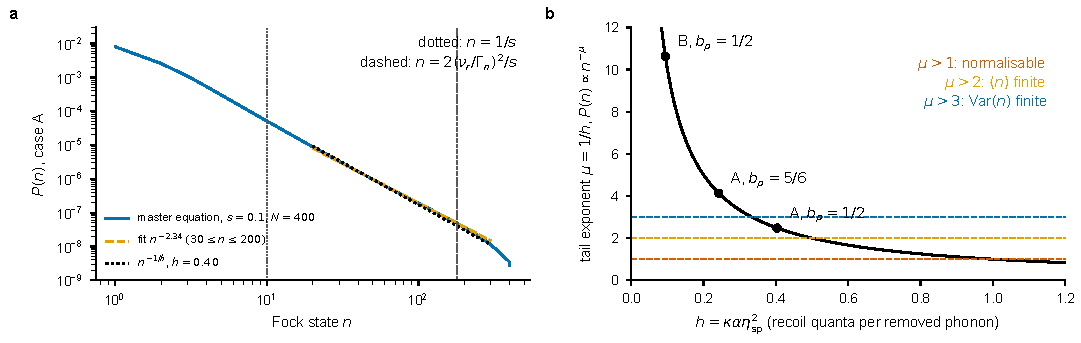
\includegraphics[width=\textwidth]{tail.pdf}
\caption{\textbf{a}, master-equation steady state at $s=0.1$ (case A, $N=400$): power-law fit over $30\le n\le200$ and the model $n^{-1/h}$. Vertical lines: $n=1/s$ and $n=2(\nur/\Gamma_n)^2/s$, the limits of regime II. \textbf{b}, tail exponent $\mu=1/h$ of Eq.~\eqref{eq:tail} and the moment thresholds, with case A ($b_p=1/2$ and $5/6$, i.e.\ D1 $F'=1$ with the probe on $F=2$) and case B.}
\label{fig:tail}
\end{figure}

\paragraph{Moments and thresholds [model, hypothesis].} If regime II extended to infinity, $\langle n^k\rangle$ would be finite only for $\mu>k+1$:
\begin{itemize}
\item $h<1/3$: mean and variance finite;
\item $1/3\le h<1/2$: ${\rm Var}(n)=\infty$; case A ($h=0.40$) lies here;
\item $1/2\le h<1$: normalisable with finite $P_0$, but $\langle n\rangle=\infty$ ("anomalous cooling");
\item $h\ge1$: no steady state, runaway heating (without regime III; with it, a hot steady state, Sec.~\ref{sec:theory}).
\end{itemize}
The mean-energy threshold $h=1/2$ is twice as strict as the naive condition $h<1$ that every cycle removes energy. In reality the tail is cut off (Sec.~\ref{sec:scales}), so the divergences are rounded into a strong sensitivity of $n_{\rm ss}$ to the cut-offs. The truncation $N$ acts as a system size: the missing part of $\langle n\rangle$ scales as $N^{2-1/h}$, so a convergence study measures $h$. This explains the slow convergence of case A, and the fast convergence of case B, where $h\approx0.09$ and the tail falls as $n^{-11}$.

\paragraph{Consequences [model].} The steady occupation is
\begin{equation}
  n_{\rm ss}=\underbrace{\Big(\frac{\Gamma}{4\Delta}\Big)^2\frac{1+h}{1-h}(1+s)}_{\text{core~\cite{morigi2000}}}+\;n_{\rm tail}(h,s,\text{cut-offs}),
\end{equation}
so that near $h\to1/2$ the tail term dominates. The ground-state population $P_0$ is the robust figure of merit, and the rate $W$ is less robust than it looks (Sec.~\ref{sec:theory}).

%=====================================================================
\section{The fast high-$n$ channel}
\label{sec:sisyphus}
%=====================================================================
\paragraph{Observation [numerics].} Beyond $s\,n\approx18$ the removal rate grows again, roughly $\propto n$, far above the narrow-line bound: 4.6$\times10^3$\,s$^{-1}$ at $n=30$ and 4.4$\times10^4$\,s$^{-1}$ at $n=200$ for $s=1$, against a plateau of $2\times10^3$\,s$^{-1}$. Plotted against $s\,n$ the drift curves collapse, and the onset sits at $s\,n=2(\nur/\Gamma_n)^2=18.0$ (Fig.~\ref{fig:regimes}).

\begin{figure}[t]
\centering
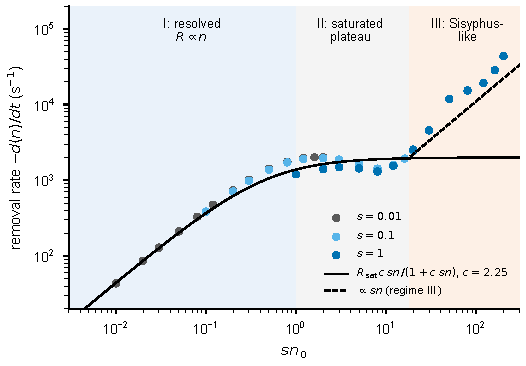
\includegraphics[width=0.62\textwidth]{regimes.pdf}
\caption{Master-equation removal rate from Fock states, case A, against $s\,n_0$ for $s=0.01$, 0.1, 1 (data from \texttt{rates\_vs\_n.dat}). Solid: Eq.~\eqref{eq:Rn} with the calibrated $c=2.25$. Dashed: growth $\propto sn$ in regime III. Shaded: regimes I (resolved, $R\propto n$), II (saturated plateau) and III (Sisyphus-like).}
\label{fig:regimes}
\end{figure}

\paragraph{Three equivalent conditions [model].} Using $\Om_R^2=s\Gamma_n^2/2$, Eq.~\eqref{eq:theta} and Eq.~\eqref{eq:dB} at the classical turning point $x_t=2x_0\sqrt n$, the onset can be written in three equivalent forms:
\begin{equation}
\begin{aligned}
  &\underbrace{\Om_R\sqrt n=\nur}_{\text{Raman splitting}=\text{trap frequency}}
  \;\Longleftrightarrow\;
  \underbrace{\tan\theta(x_t)=1}_{\text{dark state rotated by }\pi/4}\\[2pt]
  \Longleftrightarrow\;
  &\underbrace{\delta_B(x_t)-\delta_B(0)=\hbar\nur}_{\text{hill}=\text{one quantum}}
  \;\Longleftrightarrow\;
  s\,n=2\Big(\frac{\nur}{\Gamma_n}\Big)^2 .
\end{aligned}
  \label{eq:onset}
\end{equation}
More generally, $\delta_B(x_t)-\delta_B(0)=\hbar\nur\tan^2\theta(x_t)=\hbar\nur\,sn\,(\Gamma_n/\nur)^2/2$. The geometric content is visible in Fig.~\ref{fig:geometry}b: the point where $\theta=\pi/4$ falls on the turning point of $n=18/s$.

\paragraph{Mechanism [hypothesis].} For $\Om_R\sqrt n\gg\nur$ the internal state evolves faster than the atom moves, and the atom follows $\ket{D(x)}$ adiabatically. The motion couples it to the bright state non-adiabatically, with a matrix element $\propto\dot x\,\partial_x\theta$, largest near the axis where the atom is fastest. For blue detuning the bright state is shifted upwards and its shift grows with $|x|$, Eq.~\eqref{eq:dB}. The atom therefore climbs the hill while in $\ket B$, losing kinetic energy, and optical pumping at rate $\sim\Gamma_n$ returns it to $\ket D$, carrying away the potential energy. This is dark-state Sisyphus cooling, the mechanism of gray molasses~\cite{grynberg1994,weidemuller1994}. By Eq.~\eqref{eq:onset} the energy removed per cycle is of order $\hbar\nur\tan^2\theta(x_t)\propto n$. That gives $R\propto n$, unlike the one quantum per cycle of regimes I--II. At $s=1$, $n=200$ the hill is about $11\,\hbar\nur$, against the measured $\approx22$ times the plateau rate: order-of-magnitude agreement, with a missing factor that probably comes from the larger cycle rate at high $n$.

\paragraph{Relation to known physics.} The two limits are known separately. Resolved EIT cooling is the theory of Ref.~\cite{morigi2000}. Gray molasses and $\Lambda$-enhanced gray molasses~\cite{grynberg1994,weidemuller1994} have been described for trapped atoms in a unified formalism that covers resolved and unresolved sideband cooling~\cite{phatak2024}. EIT-induced friction for free atoms was proposed in Ref.~\cite{he2017}, and the high-energy breakdown and capture range of EIT cooling of ions were analysed semiclassically in Ref.~\cite{bartolotta2024}. We have not found the crossover resolved EIT $\to$ plateau $\to$ Sisyphus within one trapped atom, as a function of $n$ and $s$, in a gradient-only (node) geometry. The full texts still have to be checked before any novelty claim.

\paragraph{What is LP$_{11}$-specific.}
\begin{itemize}
\item The Sisyphus potential is the probe intensity profile, $\propto x^2$ near the node, commensurate with the harmonic trap over the whole core: one smooth hill rather than a $\lambda/2$ corrugation.
\item The crossover lies inside the thermal population. At \SI{10}{\micro K}, $\bar n\approx30$, so hot atoms are captured in regime III and finished in regime I. In tight tweezers and ion traps the crossover sits at much larger $n$.
\item The node keeps the low-$n$ regime carrier-free, so the same pair of beams provides both clean resolved cooling and Sisyphus capture.
\end{itemize}

%=====================================================================
\section{Hierarchy of scales}
\label{sec:scales}
%=====================================================================
The regimes and the physical cut-offs define a hierarchy of $n$-scales (Fig.~\ref{fig:scales}). Regime II, where the power-law tail lives, is the window $1/s<n<2(\nur/\Gamma_n)^2/s$. Its upper end is lowered by regime III. Beyond lie the cut-offs that the harmonic, single-axis model does not contain or treats only approximately:
\begin{itemize}
\item the non-linearity of the Bessel profile, at $u_{11}\,2x_0\sqrt n/a=1$, i.e.\ $n\approx470$ (case A);
\item the anharmonic frequency shift reaching $\Gamma_n$, $\tfrac38(n\hbar\nur/U_0)\nur=\Gamma_n$, i.e.\ $n\approx1380$;
\item the trap depth, $n=U_0/\hbar\nur=1552$.
\end{itemize}
The window explains the non-monotonic convergence. At $s=1$ it spans only $n\approx1$--18, so the tail is cut early and convergence is fast. At $s=0.1$ it spans $n\approx10$--180, inside the computed range, so convergence is slowest. At $s=0.01$ it lies at $n\approx100$--1800, where the population is already tiny.

\begin{figure}[t]
\centering
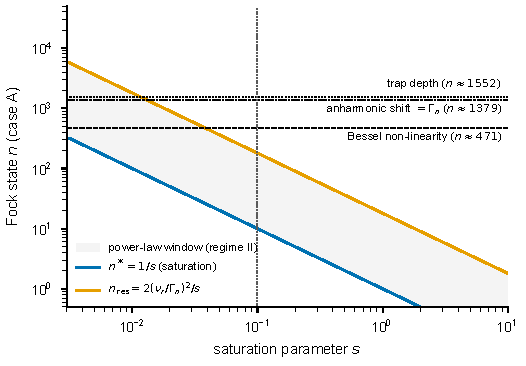
\includegraphics[width=0.62\textwidth]{scales.pdf}
\caption{Hierarchy of Fock-state scales for case A against $s$. Shaded: regime II between $n^*=1/s$ and $n_{\rm res}=2(\nur/\Gamma_n)^2/s$. Horizontal lines: Bessel non-linearity, anharmonic shift equal to $\Gamma_n$, trap depth. Dotted vertical line: $s=0.1$.}
\label{fig:scales}
\end{figure}

%=====================================================================
\section{Design map in $(\nur/\omega_{\rm rec},\,b_p)$}
%=====================================================================
Since $h=\alpha\,\omega_{\rm rec}/(b_p\nur)$, the thresholds of Sec.~\ref{sec:model} are curves in the plane of trap stiffness and branching ratio (Fig.~\ref{fig:phase}). For $^{87}$Rb D1 at $\nu_z=300$\,kHz the trap stiffness maps onto the core radius:
\begin{itemize}
\item with $b_p=1/2$, $h=1/2$ is reached at $a\approx19\,\mu$m and $h=1$ at $a\approx37\,\mu$m;
\item with $b_p=5/6$ (D1, $F'=1$, probe on $F=2$) the same thresholds move to $a\approx31\,\mu$m and $62\,\mu$m.
\end{itemize}
Case A ($a=15\,\mu$m, $h=0.40$) lies between $h=1/3$ and $1/2$; the $b_p=5/6$ configuration moves it to $h=0.24$, below $1/3$; case B lies at $h=0.09$.

\begin{figure}[t]
\centering
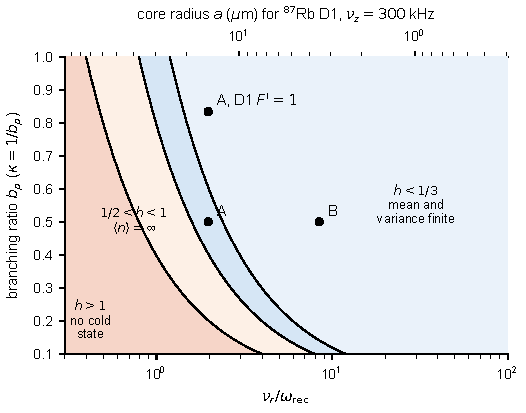
\includegraphics[width=0.62\textwidth]{phase.pdf}
\caption{Regions of the model tail in the plane of trap stiffness $\nur/\omega_{\rm rec}$ and branching ratio $b_p$, with $h=\alpha\omega_{\rm rec}/(b_p\nur)$. Lines: $h=1/3$, $1/2$, 1. The narrow band between the $h=1/3$ and $h=1/2$ lines is where only the variance diverges. Points: case A with $b_p=1/2$ and $5/6$, case B. Top axis: core radius for $^{87}$Rb D1 with $\nu_z=300$\,kHz.}
\label{fig:phase}
\end{figure}

%=====================================================================
\section{Theory of the $h$ regimes and figures of merit}
\label{sec:theory}
%=====================================================================
Nothing in this section requires a new simulation; the tests use stored data (Fig.~\ref{fig:fom}). The thresholds of Sec.~\ref{sec:model} are three values of $h$ ($\tfrac13$, $\tfrac12$, 1), which separate four windows.

\paragraph{Closed form with the fast channel [model].} In regime III the measured diffusion stays close to the plateau law while the drift grows: from $n=20$ to 200 at $s=1$ the diffusion follows $n$ within a factor 2, while the drift grows by a factor 17, and $r(n)$ rises roughly linearly (Fig.~\ref{fig:fom}b). So the photon rate is nearly unchanged and each cycle removes more energy, which is what the light-shift hill predicts [numerics]. Adding this to the drift,
\begin{equation}
  v(n)=-R\Big(1-h+\frac{n}{n_c}\Big),\quad D(n)=h\,n\,R,\quad n_c=\frac{2(\nur/\Gamma_n)^2}{s}\simeq\frac{2(\Delta/\Gamma)^2}{s},
\end{equation}
gives, for $n\gg1$ and $n\gg1/s$,
\begin{equation}
  P(n)\propto n^{-1/h}\,e^{-n/n_x},\qquad n_x=h\,n_c .
  \label{eq:gamma}
\end{equation}
This holds for all $h$, also above 1. Compared with the data, the form is right but the scale is about twice too small: fits give $n_x\approx16$ at $s=1$ against $h\,n_c=7$, and at $s=0.1$ the tail steepens only above $n\approx200$. The linear law also misses the sharp onset near $n_c$ seen in Fig.~\ref{fig:fom}b. Treat $n_x$ as $\simeq2h\,n_c$, to be derived from the semiclassical friction.

\paragraph{The tail is a Fokker--Planck tail [numerics].} Using only the measured $v$ and $D$ in $P\propto D^{-1}\exp\int v/D$, with no fit other than the normalisation, reproduces the master-equation tail for $n\gtrsim5$ (Fig.~\ref{fig:fom}a). This removes the earlier open question of why the exponent is close to $1/h$. Below $n\approx5$ the description fails, as a single jump, $\sqrt{2hn}$, is then comparable with $n$: the predicted slope $-1-1/h=-3.5$ for $n<1/s$ is not seen (measured $-2.4$ for $2\le n\le6$ at $s=0.1$).

\paragraph{Moments as functions of $h$ [model].} Since the power law continues from low $n$ in practice, $P(n)\simeq P_1\,n^{-\mu}e^{-n/n_x}$ with $\mu=1/h$ gives
\begin{equation}
  1-P_0\simeq P_1\,\zeta(\mu),\qquad
  \langle n\rangle\simeq P_1\sum_n n^{1-\mu}e^{-n/n_x},\qquad
  \langle n^2\rangle\simeq P_1\sum_n n^{2-\mu}e^{-n/n_x}.
\end{equation}
The ratio $\langle n\rangle/(1-P_0)$ is 1 for a two-level population and grows with the tail, so it is a single-number diagnostic. Measured for case A, it is 2.5 at $s=0.1$ and 3.3 at $s=1$. As a check on the variance window: the variance at $s=0.1$ grows from 0.41 ($N=160$) to 0.67 ($N=400$), i.e.\ as $N^{0.54}$, against the predicted $N^{3-1/h}=N^{0.5}$. So the variance of case A is indeed set by the cut-off, while the mean only drifts (0.0316 to 0.0327).

\paragraph{The thresholds are crossovers, with a width set by $\Delta$ [model].} The window between the saturation scale $1/s$ and $n_c$ spans a factor $\rho=2(\Delta/\Gamma)^2$, independent of $s$. A moment changes behaviour when $|k+1-\mu|\ln\rho\sim1$, so each threshold has the width
\begin{equation}
  \delta h\simeq\frac{h^2}{\ln\rho} ,
  \label{eq:width}
\end{equation}
that is $\delta h=0.09$ at $h=\tfrac12$ for $\Delta=3\Gamma$ ($\rho=18$) and 0.04 for $\Delta=12\Gamma$ ($\rho=288$). Case A ($h=0.40$) therefore lies at the edge of the $h=\tfrac12$ crossover at $\Delta=3\Gamma$. A sharp test of a threshold needs large $\Delta$ with $N\gg n_c$, which is why the convergence worsens with $\Delta$. At large $\Delta$, neighbouring excited levels also change the branching ratio, so $h$ must be computed with the effective value: D2 $F'=2$, probe on $F=1$, at $12\Gamma$ has $b_{\rm eff}=0.37$, hence $h\approx0.57$, in the window where $\langle n\rangle$ is set by the cut-off, and indeed $n_{\rm ss}=0.038$, 0.050, 0.059, 0.069 at $N=80$, 160, 250, 400 (\texttt{lines\_nconv\_d2.dat}).

\paragraph{The four windows [model].} Using $h\simeq0.0134\,(a/\micro{\rm m})/b_p$ for $^{87}$Rb D1 at $\nu_z=300$\,kHz:

\begin{center}\small
\begin{tabularx}{\textwidth}{@{}llllX@{}}
\toprule
Window & Statistics & $a$ ($\micro$m), $b_p=\tfrac12$ & $b_p=\tfrac56$ & Examples\\
\midrule
$h<\tfrac13$ & mean, variance finite & $<12$ & $<21$ & B ($h=0.09$); A with $b_p=\tfrac56$ ($0.24$)\\
$\tfrac13<h<\tfrac12$ & variance set by cut-off & 12--19 & 21--31 & A with $b_p=\tfrac12$ ($0.40$)\\
$\tfrac12<h<1$ & mean set by cut-off, $P_0$ finite & 19--37 & 31--62 & D2 $F'=2$ at $12\Gamma$ ($0.57$)\\
$h>1$ & no cold state, hot steady state & $>37$ & $>62$ & A with $b_p=\tfrac16$ ($1.21$)\\
\bottomrule
\end{tabularx}
\end{center}

\paragraph{Above $h=1$ there is no runaway [model, partly tested].} The drift vanishes at $n=(h-1)n_c$, and Eq.~\eqref{eq:gamma} is integrable at low $n$ for $h>1$, with
\begin{equation}
  \langle n\rangle=n_x\frac{\Gamma(2-1/h)}{\Gamma(1-1/h)}=(h-1)\,n_c ,
  \label{eq:hot}
\end{equation}
the same value. So $h=1$ does not end the steady state: it ends ground-state cooling, and the atoms settle at a temperature set by the balance of recoil and Sisyphus cooling. For $b_p=\tfrac16$ in case A ($h=1.21$), Eq.~\eqref{eq:hot} gives 3.8 at $s=1$ against the converged $n_{\rm ss}=2.69$, the right order. However, it predicts $0.76$ at $s=5$ against 1.44, so the expected $1/s$ scaling is not confirmed where $n_c$ approaches $1/s$; and at $s=0.1$ it predicts $\approx38$, while $n_{\rm ss}$ is still rising at $N=250$ (4.18). The naive threshold ``no steady state at $h\ge1$'' of Sec.~\ref{sec:model} applies only in the absence of regime III.

\paragraph{Why $W$ fails in a heavy tail [model, supported by data].} From $\ket{g_p,1}$, $\langle n\rangle$ falls quickly to the core value and then \emph{rises} slowly to $n_{\rm ss}$ as recoil fills the tail. With $n_{\rm ss}=n_{\rm core}+n_{\rm tail}$,
\begin{equation}
  \frac{1-n_{\rm ss}}{W}=\int_0^\infty\big(\langle n\rangle-n_{\rm ss}\big)dt\simeq\frac{1-n_{\rm core}}{W_c}-\frac{n_{\rm tail}}{\lambda},
\end{equation}
with $W_c$ the true decay rate of the core and $\lambda$ the slow filling rate. The negative term raises $W$, and $W\to\infty$ and then $W<0$ when $n_{\rm tail}/\lambda$ reaches $1/W_c$. This explains three observations: the pole and sign change of $W$ versus $\delta_{\rm e}$ near $n_{\rm ss}\approx0.2$ (\texttt{lines\_d2scan.dat}), the negative $W$ at $\Delta=\Gamma$, and the runaway $W=206$, 207, 237, 399, 1254\,s$^{-1}$ at $N=80$, 160, 250, 400, 550 for D2 $F'=2$ at $12\Gamma$ while $n_{\rm ss}$ changes by only 56\%. There, $\Delta(1/W)/\Delta n_{\rm ss}$ gives $1/\lambda\approx0.5$\,s, of the order of the time to reach $n\sim300$ at the plateau rate.

\paragraph{The ground-state rate [numerics].} A well-behaved rate is that of the ground-state population, with $P_0(0)=0$ from $\ket{g_p,1}$:
\begin{equation}
  W_0^{-1}=\frac{1}{P_0^{\rm ss}}\int_0^\infty\big(P_0^{\rm ss}-P_0(t)\big)dt ,
  \label{eq:W0}
\end{equation}
in which the tail enters through its weight ($10^{-3}$) instead of its energy. It costs one extra product with the existing solution (\texttt{solve\_banded}; \texttt{rate\_p0.dat}):

\begin{center}\small
\begin{tabularx}{\textwidth}{@{}Xll@{}}
\toprule
Point & $W$ (s$^{-1}$) & $W_0$ (s$^{-1}$)\\
\midrule
Case A, $s=1$, $N=20$, 40, 120 & 1319, 1544, 1614 & 2188, 2220, 2225\\
Case A, $s=0.01$, 0.1, 5 (converged $N$) & 42, 338, 3321 & 51, 451, 4555\\
$b_p=\tfrac56$, $s=0.1$, 1, 5 & 515, 2941, 4680 & 551, 3441, 6601\\
D2 $F'=2$, $g_p=2$, $12\Gamma$, $N=80$, 160, 250, 400 & 206, 207, 237, 399 & 507, 507, 509, 511\\
D2 $F'=2$, $g_p=2$, $3\Gamma$, $\delta_{\rm e}=-0.05$, 0, 0.09, 0.13, 0.3 & $-2850$, 4587, 1839, 1629, 1123 & 1395, 1695, 2143, 2225, 1819\\
\bottomrule
\end{tabularx}
\end{center}

So $W_0$ is converged where $W$ is not, and it has a real maximum in $\delta_{\rm e}$ where $W$ has a pole. The rise of $W$ with $N$ in the fibre paper's case A is therefore a tail effect: $W$ changes by 22\% from $N=20$ to 120, $W_0$ by 1.7\%.

$W$ and $W_0$ do not measure the same thing, however, and $W$ is not simply an overestimate. An earlier version of this section suggested that the true rate lies below $W$, using the drift from $n_0=1$ (1199\,s$^{-1}$ at $s=1$) as a proxy; $W_0$ lies \emph{above} $W$, by a factor 1.2 even at weak probe, where the tail is light. A possible reading [hypothesis]: $W$ integrates energy, so a recoil excursion to high $n$ costs it a long time, whereas $W_0$ only asks how soon the atom reaches $n=0$. At $s=1$ the three numbers answer three questions: net energy removal from $n=1$ (1199), integrated energy relaxation (1614), arrival in the ground state (2225)\,s$^{-1}$. For the applications below, where $P_0$ matters, $W_0$ is the relevant one. Whether $1/W_0$ gives the time to reach $P_0$ from a thermal state has still to be checked with the time evolution.

\paragraph{Figures of merit from applications [model].} The hyperfine coherence of an atom in $\ket n$ acquires a phase at the differential light shift, $2\pi\epsilon nT$, with $\epsilon=\delta_{\rm diff}\hbar\nur/2U_0=0.26$\,Hz per quantum per axis for case A and $\delta_{\rm diff}=800$\,Hz (the paper's value; 1.1\,Hz for case B). An ensemble then has the coherence $|\phi(T)|^2$ for two equal axes, with $\phi(T)=\sum_nP(n)e^{2\pi i\epsilon nT}$, the characteristic function of $P(n)$. All the statistics enter through this one function (Fig.~\ref{fig:fom}c):
\begin{itemize}
\item at short $T$, $1-|\phi|^2\simeq(2\pi\epsilon T)^2{\rm Var}(n)$, so the variance matters first;
\item for $\epsilon T\gtrsim\tfrac12$ the excited atoms dephase while the ground-state atoms do not, so $|\phi|^2$ settles around $P_0^2$, with a modulation of order $2P_0P_1$, and does not decay further (Fig.~\ref{fig:fom}c: 0.97, 0.89, 0.67 at $T=1$\,s for $s=0.1$, 1, 5, with $P_0^2=0.974$, 0.909, 0.712).
\end{itemize}
So dephasing from a cold distribution is a loss of contrast, not a decay. Harmonic revivals at $T=1/\epsilon$ ($\approx3.9$\,s) would be washed out by anharmonicity, which is not included. A spin echo would remove this static part; heating during storage would not be removed.

\begin{center}\small
\begin{tabularx}{\textwidth}{@{}lXl@{}}
\toprule
Application & What limits it & Figure of merit, threshold\\
\midrule
Spin-wave memory, long $T$ & fraction of atoms that keep their phase; retrieval efficiency $\propto|\phi|^4\to P_0^4$ for two axes & $P_0$; $h=1$ (and $1-P_0\propto P_1\zeta(\mu)$)\\
Interferometer, clock & shot-to-shot noise of the sample mean, $\sigma_\varphi=2\pi\epsilon T\sqrt{2{\rm Var}(n)/N_a}$, against the quantum projection noise $1/\sqrt{N_a}$; contrast $P_0^2$ & $\sigma_n$ at fixed $P_0$; $h=\tfrac13$\\
Mean shifts, thermometry & systematic shift $\propto\langle n\rangle$ & $\langle n\rangle$; $h=\tfrac12$\\
Waveguide QED, Rydberg & spread of coupling from the radial position, with hot atoms near the wall in the worst case & $P(n>n_{\rm cut})$\\
Any repeated protocol & preparation time, scattered photons & $t_{\rm prep}$, $N_{\rm ph}$\\
\bottomrule
\end{tabularx}
\end{center}

For the interferometer, $\sigma_\varphi$ reaches the projection noise at $T_{\rm QPN}=[2\pi\epsilon\sqrt{2{\rm Var}(n)}]^{-1}$, independent of $N_a$: 0.53\,s at $s=0.1$ and 0.36\,s at $s=1$ for case A (the first still falling with $N$), without echo. This is the practical meaning of the variance window, and it is only relevant for such long $T$. The numbers depend on $\delta_{\rm diff}$, which is much smaller in a magic-like configuration.

The recommended single measure is $t_{\rm prep}(P_0^\ast)$, the time to reach a target $P_0^\ast$ per axis from the pre-trap distribution, with $\sigma_n$ reported where metrology matters. $\langle n\rangle$ alone is misleading: in case A at $s=0.1$, $3\times10^{-4}$ of the atoms ($n>10$) carry 27\% of $\langle n\rangle$ and 89\% of $\langle n^2\rangle$. $W$ alone is also misleading, as shown above.

\paragraph{Best configuration [model].} With the core infidelity $\varepsilon=(\Gamma/4\Delta)^2\frac{1+h}{1-h}(1+s)$ of Sec.~\ref{sec:model}, a rate $\propto(1-h)b_p\Gamma_n\frac{s}{1+s}$ and $\Gamma_n=\Gamma\nur/\Delta$, the rate at a given target infidelity is
\begin{equation}
  W(\varepsilon)\propto\nur\sqrt\varepsilon\;\underbrace{b_p\frac{(1-h)^{3/2}}{(1+h)^{1/2}}}_{Q}\;\frac{s}{(1+s)^{3/2}} .
\end{equation}
\begin{itemize}
\item $s$: the factor peaks at $s=2$ with the core alone. The tail, ignored here, raises $1-P_0$ at large $s$ (the master equation gives $P_0=0.844$ at $s=5$), so the practical optimum is lower, $s\sim1$ in the last stage.
\item $b_p$: at fixed trap, $Q$ favours large $b_p$ twice, directly and through $h$. Case A: $Q=0.20$ for $b_p=\tfrac12$, $0.50$ for $b_p=\tfrac56$, a factor 2.5; the master equation gives 1.8 in $W$ and 1.55 in $W_0$, so this estimate overstates the gain.
\item $\nur$: the rate grows with $\nur$ and $h$ falls, so a stiffer trap always helps; the limit is the fibre (loading, wall effects), not the cooling.
\item $\Delta$: set by the target, $\Delta/\Gamma\simeq\frac14\sqrt{\frac{1+h}{1-h}\frac{1+s}{\varepsilon}}$. For $h=0.24$, $s=1$: $4.5\Gamma$ for $\varepsilon=0.01$ and $14\Gamma$ for $\varepsilon=10^{-3}$. Stored three-level values give $n_{\rm ss}=0.013$ and 0.005 at $5\Gamma$ and $8\Gamma$, about 1.6 times the core estimate.
\end{itemize}
The candidate in $^{87}$Rb is therefore \textbf{D1, $F'=1$, probe on $F=2$} ($b_p=\tfrac56$, $h=0.24$ in case A, below all the thresholds up to $a\approx21\,\micro$m), with $\Delta\approx5$--$8\Gamma$, $s\sim1$ as the last stage. The D1/D2 scan with $\delta_{\rm e}$ selected on $W_0$ supports this (all excited levels, sign $+1$, $s=1$): $P_0=0.990$ at $5\Gamma$ with $W_0=1.9\times10^3$\,s$^{-1}$, as the estimate $4.5\Gamma$ predicts, whereas $b_p=\tfrac12$ reaches $P_0=0.99$ only near $6\Gamma$, with $W_0\approx1.0\times10^3$\,s$^{-1}$, about half the rate. It is limited by the Zeeman dark states of $F=2\to F'=1$, which the model does not contain; this is the main open risk. $W_0$ itself is meaningful only for cold states: for $P_0\lesssim0.85$ it can be negative or misleadingly large, so it must be read together with $P_0$.

For hot atoms the theory suggests a ramp [hypothesis]: at large $s\,n$ the fast channel removes energy efficiently, so one can begin with large $s$ and small $\Delta$, and reduce $s$ as $\langle n\rangle$ falls, ending at the settings above. This is the staged protocol of the fibre paper extended by regime III. Lowering the trap depth to spill the tail could also remove the atoms that carry the variance at a small cost in atom number, as they are a fraction $<10^{-3}$. Neither has been simulated.

\begin{figure}[t]
\centering
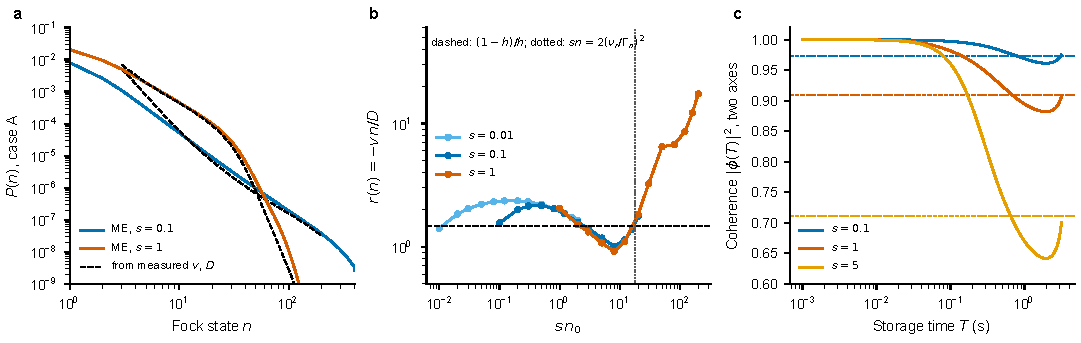
\includegraphics[width=\textwidth]{fom.pdf}
\caption{Stored case-A data against the theory. \textbf{a}, master-equation $P(n)$ and the Fokker--Planck form built from the measured drift and diffusion, normalised at $n=12$ ($s=0.1$) and $n=5$ ($s=1$); no fit parameters otherwise. \textbf{b}, local exponent $r=-v\,n/D$ with $D=\tfrac12d{\rm Var}/dt$: near $(1-h)/h$ on the plateau, rising in regime III. \textbf{c}, coherence for two equal axes from the steady $P(n)$, $\epsilon=0.26$\,Hz; dashed: $P_0^2$.}
\label{fig:fom}
\end{figure}

\paragraph{How to study the windows numerically, when simulations resume.} In order of cost:
\begin{enumerate}
\item Report $W_0$ and $\langle n\rangle/(1-P_0)$ next to $W$, $n_{\rm ss}$ in the remaining scans; $\delta_{\rm e}$ in the D1/D2 study is already selected on $W_0$.
\item A chain for $P(n)$ with the exact recoil kernel and measured $R(n)$ ($N$ up to several thousand, cheap), with regime III on and off: thresholds without cut-off, then their rounding. This is the only way to test the sharp thresholds, since the master equation stops at $N\approx550$ with 11\,GB.
\item Master equation at $h=0.1$, 0.25, 0.33, 0.4, 0.5, 0.6, 0.8, 1, 1.2, reached in two ways, by $\nur/\omega_{\rm rec}$ at $b_p=\tfrac12$ and by $b_p$ at fixed trap, at $s=1$, $\Delta=8\Gamma$ ($\rho=128$, $N=400$). Equal tails at equal $h$ test universality. The band $B$ must be rechecked in regime III, where $\Om_R\sqrt n>\nur$ may widen the coherences.
\item Banded time evolution for $t_{\rm prep}(P_0^\ast)$ from thermal states, with $P_0(t)$ added to the output: about 4\,min per point at $N=400$, for $(\Delta,s,b_p)$ and for ramps.
\end{enumerate}

%=====================================================================
\section{Predictions and tests}
%=====================================================================
\begin{enumerate}
\item \textbf{Universality of the tail.} Tails for different $(\nur/\omega_{\rm rec},b_p,s)$ at equal $h$ should collapse. Fit the exponent against $h$ by scanning the reduced parameter $\nur/\omega_{\rm rec}$ with the banded solver.
\item \textbf{Finite-size scaling.} The missing part of $n_{\rm ss}$ should scale as $N^{2-1/h}$, and the scaling exponent should agree with the tail exponent.
\item \textbf{Thresholds.} Check the rounding of Eq.~\eqref{eq:width} and, above $h=1$, the hot steady state of Eq.~\eqref{eq:hot} instead of a runaway.
\item \textbf{Sisyphus channel.}
\begin{itemize}
\item The onset should move as $2(\nur/\Gamma_n)^2/s\simeq2(\Delta/\Gamma)^2/s$ when $\Delta/\Gamma$ is varied.
\item Red detuning should turn regime III into heating while regimes I--II survive.
\item The high-$n$ rate should scale like a Sisyphus friction, with $\Om_c$, $\Delta$ and $\Gamma$, not with $\Gamma_n$.
\item The bright-state population should rise at high $n$, as the atom follows the dark state only adiabatically.
\end{itemize}
\item \textbf{Semiclassical model.} Compute the friction and momentum diffusion of an atom moving through the LP$_{11}$ gradient from linear response of the optical Bloch equations, and compare with the master-equation drift in regime III.
\item \textbf{Capture.} Banded time evolution from thermal states ($\bar n\approx30$, $N\approx400$) should give the true capture time from \SI{10}{\micro K}, which may be much shorter than the rate-model estimate because of regime III.
\item \textbf{Beyond the minimal model.} Treat the recoil with its exact Franck--Condon kernel in a master equation for $P(n)$ in place of the Fokker--Planck form, which fails at $n\lesssim5$ where single jumps are comparable with $n$.
\item \textbf{Rate definitions.} Check $1/W_0$ against the time to reach $P_0$ from thermal states, and the origin of the factor $W_0/W\approx1.2$ at weak probe.
\end{enumerate}

\begin{thebibliography}{99}
\bibitem{morigi2000} G.~Morigi, J.~Eschner and C.~H.~Keitel, Ground state laser cooling using electromagnetically induced transparency, Phys.\ Rev.\ Lett.\ \textbf{85}, 4458 (2000).
\bibitem{cirac1992} J.~I.~Cirac, R.~Blatt, P.~Zoller and W.~D.~Phillips, Laser cooling of trapped ions in a standing wave, Phys.\ Rev.\ A \textbf{46}, 2668 (1992).
\bibitem{reiter2012} F.~Reiter and A.~S.~S{\o}rensen, Effective operator formalism for open quantum systems, Phys.\ Rev.\ A \textbf{85}, 032111 (2012).
\bibitem{kesten1973} H.~Kesten, Random difference equations and renewal theory for products of random matrices, Acta Math.\ \textbf{131}, 207 (1973).
\bibitem{sornette1998} D.~Sornette, Multiplicative processes and power laws, Phys.\ Rev.\ E \textbf{57}, 4811 (1998).
\bibitem{bardou1994} F.~Bardou, J.-P.~Bouchaud, O.~Emile \emph{et al.}, Subrecoil laser cooling and Lévy flights, Phys.\ Rev.\ Lett.\ \textbf{72}, 203 (1994).
\bibitem{grynberg1994} G.~Grynberg and J.-Y.~Courtois, Proposal for a magneto-optical lattice for trapping atoms in nearly-dark states, Europhys.\ Lett.\ \textbf{27}, 41 (1994).
\bibitem{weidemuller1994} M.~Weidemüller, T.~Esslinger, M.~A.~Ol'shanii \emph{et al.}, A novel scheme for efficient cooling below the photon recoil limit, Europhys.\ Lett.\ \textbf{27}, 109 (1994).
\bibitem{phatak2024} S.~S.~Phatak, K.~N.~Blodgett, D.~Peana, M.~R.~Chen \emph{et al.}, A generalized theory for optical cooling of a trapped atom with spin, Phys.\ Rev.\ A \textbf{110}, 043116 (2024).
\bibitem{he2017} P.~He, P.~M.~Tengdin, D.~Z.~Anderson and A.~M.~Rey, Sub-Doppler laser cooling using electromagnetically induced transparency, Phys.\ Rev.\ A \textbf{95}, 053403 (2017).
\bibitem{bartolotta2024} J.~P.~Bartolotta, B.~Estey, M.~Foss-Feig, D.~Hayes \emph{et al.}, Laser cooling trapped-ion crystal modes beyond the Lamb--Dicke regime, arXiv:2411.18818 (2024).
\end{thebibliography}

\end{document}
